\documentclass[14pt]{article}
\usepackage{amsmath}
\usepackage{latexsym}
\usepackage{amsfonts}
\usepackage[normalem]{ulem}
\usepackage{soul}
\usepackage{array}
\usepackage{amssymb}
\usepackage{extarrows}
\usepackage{graphicx}
\usepackage[backend=biber,
style=numeric,
sorting=none,
isbn=false,
doi=false,
url=false,
]{biblatex}\addbibresource{bibliography-biblatex.bib}

\usepackage{subfig}
\usepackage{wrapfig}
\usepackage{txfonts}
\usepackage{wasysym}
\usepackage{enumitem}
\usepackage{adjustbox}
\usepackage{ragged2e}
\usepackage[svgnames,table]{xcolor}
\usepackage{tikz}
\usepackage{longtable}
\usepackage{changepage}
\usepackage{setspace}
\usepackage{hhline}
\usepackage{multicol}
\usepackage{tabto}
\usepackage{float}
\usepackage{multirow}
\usepackage{makecell}
\usepackage{fancyhdr}
\usepackage[toc,page]{appendix}
\usepackage[hidelinks]{hyperref}
\usetikzlibrary{shapes.symbols,shapes.geometric,shadows,arrows.meta}
\tikzset{>={Latex[width=1.5mm,length=2mm]}}
\usepackage{flowchart}\usepackage[paperheight=11.0in,paperwidth=8.5in,left=1.0in,right=1.0in,top=1.5in,bottom=1.5in,headheight=1in]{geometry}
\usepackage[utf8]{inputenc}
\usepackage[T1]{fontenc}
\TabPositions{0.5in,1.0in,1.5in,2.0in,2.5in,3.0in,3.5in,4.0in,4.5in,5.0in,5.5in,6.0in,}

\urlstyle{same}




% 1) Section
% 1.1) SubSection
% 1.1.1) SubSubSection
% 1.1.1.1) Paragraph
% 1.1.1.1.1) Subparagraph


\setcounter{tocdepth}{5}
\setcounter{secnumdepth}{5}





\setlistdepth{9}
\renewlist{enumerate}{enumerate}{9}
		\setlist[enumerate,1]{label=\arabic*)}
		\setlist[enumerate,2]{label=\alph*)}
		\setlist[enumerate,3]{label=(\roman*)}
		\setlist[enumerate,4]{label=(\arabic*)}
		\setlist[enumerate,5]{label=(\Alph*)}
		\setlist[enumerate,6]{label=(\Roman*)}
		\setlist[enumerate,7]{label=\arabic*}
		\setlist[enumerate,8]{label=\alph*}
		\setlist[enumerate,9]{label=\roman*}

\renewlist{itemize}{itemize}{9}
		\setlist[itemize]{label=$\cdot$}
		\setlist[itemize,1]{label=\textbullet}
		\setlist[itemize,2]{label=$\circ$}
		\setlist[itemize,3]{label=$\ast$}
		\setlist[itemize,4]{label=$\dagger$}
		\setlist[itemize,5]{label=$\triangleright$}
		\setlist[itemize,6]{label=$\bigstar$}
		\setlist[itemize,7]{label=$\blacklozenge$}
		\setlist[itemize,8]{label=$\prime$}

\setlength{\topsep}{0pt}\setlength{\parskip}{9.38pt}
\setlength{\parindent}{0pt}




\renewcommand{\arraystretch}{1.3}






\begin{document}
\begin{Center}
CSE 344 HW1 REPORT
\end{Center}

\vspace{\baselineskip}
{\fontsize{16pt}{19.2pt}\selectfont \textbf{a) How am I Solved This Problem}}

\vspace{\baselineskip}
\textit{Steps:}
1- First, I divide problem into chunks, 
2- I started with the easy stuff such as reading command line options with getopt (), writing filename comparator with ability to support regex etc.
3- Then I wrote crucial function for homework to check are the attributes of files match between target file data and traversed file data. 
4- After all these things are ready. I wrote a function to traverse all the files within specified pathname recursively, I can print all files on the screen with this function but it’ s hard to print the ‘found’ files. Because of the need of memorizing all the found files programmatically.
5- I hold the full pathnames of found files in a 2D array in mentioned above function (step 4), I have decided to write separate function to print all the tree structure with the found files.
6- Two helper functions are created to complete printing of found files on the screen.
7- Then I made minor corrections on the functions like case-insensitivity.
8- I worked on memory management for hours, because when I searched for filetype as f (-t f) in the root directory, it found 320 thousand files on my system and I wanted to print all of these on the screen in a tree structure. I believe, finally I optimized memory requirement of my program.

\vspace{\baselineskip}
{\fontsize{18pt}{21.6pt}\selectfont \textbf{b) Design Decisions}}
1) While traversing file system, my program compare each file with the sought file, and if there is a match which we are looking for, program stored found file’s pathname into a 2D char array. when the all traversing process has ended, Program starts printing those found files with the help of their pathnames in 2D char array.
2) In printing process, firstly, program prints first found file, Meanwhile, I kept the printed dir names and filenames in 3D char array. If the next found file has one of the dir names printed on the screen before, it will not print it again, it will print "--" instead.
3) I had to keep the arrays in the heap in the recursive function, since  it was recursive, stack was overflowing.

\vspace{\baselineskip}
{\fontsize{18pt}{21.6pt}\selectfont \textbf{c) Requirements}}
{\fontsize{18pt}{21.6pt}\selectfont \textbf{Satisfied}}
1) There is no warning with respect to -Wall flag
\setlength{\parskip}{0.0pt}
2) If the required command line arguments are missing/invalid, my program prints usage
\setlength{\parskip}{9.38pt}
information and exits.



\begin{figure}[H]
	\begin{Center}
		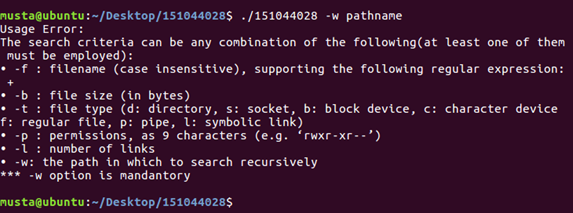
\includegraphics[width=5.97in,height=2.22in]{./media/image1.png}
	\end{Center}
\end{figure}


\vspace{\baselineskip}



\vspace{\baselineskip}3) There is no memory leak with respect to valgrind



\begin{figure}[H]
	\begin{Center}
		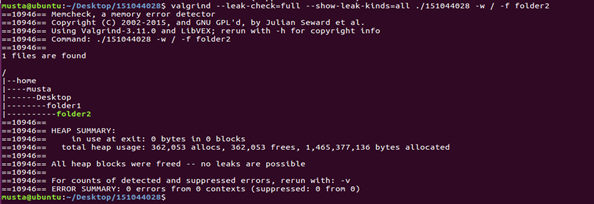
\includegraphics[width=6.18in,height=2.12in]{./media/image2.png}
	\end{Center}
\end{figure}




\vspace{\baselineskip}4) Shows Results as a tree structure according to specified option, green ones found files



\begin{figure}[H]
	\begin{Center}
		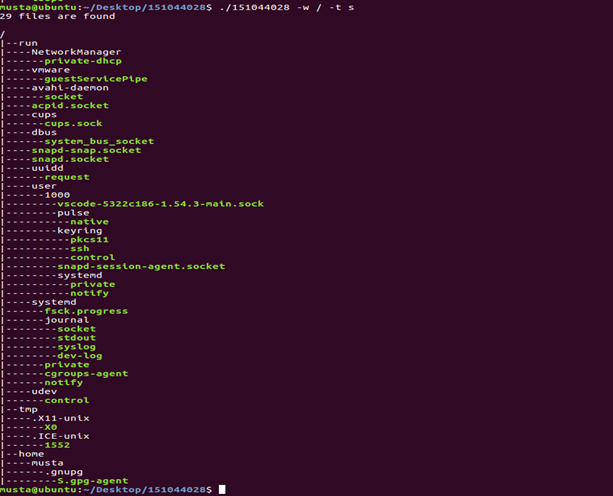
\includegraphics[width=5in,height=4.5in]{./media/image3.png}
	\end{Center}
\end{figure}




\vspace{\baselineskip}
\vspace{\baselineskip}

\vspace{\baselineskip}

\vspace{\baselineskip}

\vspace{\baselineskip}

\vspace{\baselineskip}

\vspace{\baselineskip}

\vspace{\baselineskip}

\vspace{\baselineskip}

\vspace{\baselineskip}

\vspace{\baselineskip}

\vspace{\baselineskip}

\vspace{\baselineskip}

\vspace{\baselineskip}





5) regexp and case insensitivity works fine

\vspace{\baselineskip}




\begin{figure}[H]
	\begin{Center}
		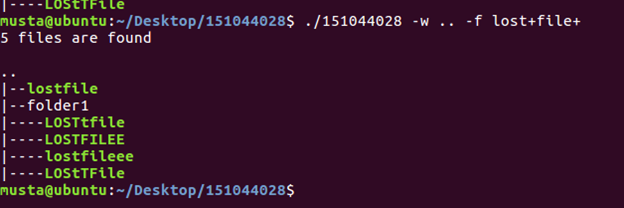
\includegraphics[width=6.5in,height=2.16in]{./media/image4.png}
	\end{Center}
\end{figure}






6) SIGINT handler works as expected




\begin{figure}[H]
	\begin{Center}
		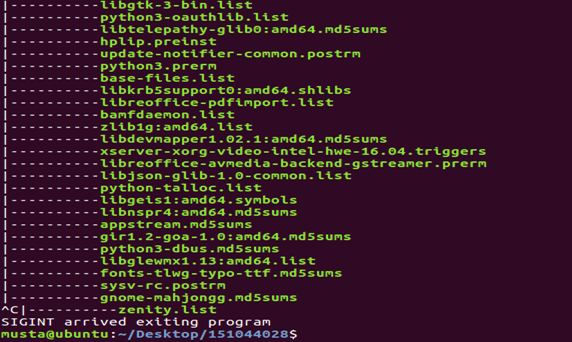
\includegraphics[width=5.96in,height=3.57in]{./media/image5.png}
	\end{Center}
\end{figure}





\vspace{\baselineskip}{\fontsize{18pt}{21.6pt}\selectfont \textbf{Unsatisfied}}
1- finding symbolic links with\  ./program -w / -t l, I block symbolic links because it causes so much repetation of paths but when I block them I cant found soft links with above commands. 
\printbibliography
\end{document}
